\if0
\documentclass[12pt, a4paper, fleqn]{jreport}

\usepackage{graduatethesis}
\usepackage{listings,jlisting}
\usepackage{cite}
\usepackage{here}


\begin{document}
\setcounter{tocdepth}{2}
\setlength{\mathindent}{0zw}
\pagenumbering{roman}
\pagenumbering{arabic}
\setcounter{totalnumber}{3}
\setcounter{topnumber}{3}
\renewcommand{\topfraction}{0.99}
\renewcommand{\bottomfraction}{0.99}
\renewcommand{\textfraction}{0.0}

\lstset{
  basicstyle={\ttfamily},
  breaklines=true,
  columns=[l]{fullflexible},
  lineskip=-0.5zw,
}

\setlength{\textwidth}{\paperwidth}   %%本文を用紙の横サイズにする
\addtolength{\textwidth}{-2in}         %それを2インチ引く
\setlength{\textheight}{\paperheight} %%本文を用紙の縦サイズにする
\addtolength{\textheight}{-2in}        %それを2インチ引く
\setlength{\topmargin}{0pt}            %ページ上端の余白を消す
\addtolength{\topmargin}{-\headheight} %(ページ上端の余白)-(ヘッダーの高さ)
\addtolength{\topmargin}{-\headsep}    %                  -(ヘッダーと本文の余白)
\setlength{\oddsidemargin}{0pt}       %%奇数(右)ページの左余白消す
\setlength{\evensidemargin}{0pt}      %%偶数(左)ページの左余白を消す


\fi



\chapter{数値実験}
本章では,本研究で作成した数理計画モデルと,実際に使用している関西大学の理工系全学部の時間割を用いて,様々な教室割当を行った実験内容と結果について述べる.

本研究では,以下の実験を行った.
\begin{itemize}
\item 予備実験1: サンプルデータを用いた,各制約式が正しく機能するかを確かめる実験
\item 予備実験2:春学期火曜午前のデータを用いた,移動時間の制限を300秒とする確認実験
\item 本実験1:移動時間の制限を小さくしていき,最大移動時間の最小値を求める実験
\item 本実験2:本実験1において最大移動時間が大きいデータから原因の授業を取り除いた実験
\item 本実験3:考慮制約2の希望教室を設定した春学期火曜午前のデータを用いた実験
\end{itemize}

なお,本研究では,全ての実験においてパラメータ$pa_1 = 1$,$pa_2 = -1$,$z = 100$を与えている.
\section{計算環境}
本研究では,先行研究と同様に,最適化ソルバーIBM ILOG CPLEXの分枝限定法を用いて求解を行っている.
表\ref{kankyo}は,本研究で用いた計算環境を示している.

\begin{table}[H]
\begin{center}
\label{kankyo}
\caption{計算環境}
\scalebox{1.0}{ 
\begin{tabular}{cc}
\hline
OS & Microsoft Windows 7 Home Premium Service Pack 1\\
CPU &Intel(R) Core(TM) i5-2520M CPU @ 2.50GHz\\ 
メモリ & 8.0 GB\\
ソルバー1&GLPK 4.47\\
ソルバー2&IBM ILOG CPLEX 12.5.0.0\\
\hline
\end{tabular}
}
\end{center}
\end{table}
\section{予備実験}
\subsection{予備実験1:各制約式が正しいく機能するかを確かめる実験}
予備実験1は,ごく小さな規模のサンプルデータを用いた数値計算である.
予備実験1の目的は,モデルファイルが意図した形で展開され,制約を満たす解が得られるかどうかを確かめることである.

表\ref{b:normal_information}~表\ref{f:normal_information}は,使用したサンプルデータの内容を示している.\\

\begin{table}[H]
\caption{サンプルデータ:教室毎の定員}
\label{b:normal_information}
\begin{center}
\begin{tabular}{c|ccccccc}
\hline
教室 & 101 & 102 & 103 & 104 & 105 & 106 & 107 \\
定員 & 150 & 150 & 180 & 100 & 180 & 180 & 100  \\
\hline
\end{tabular}
\end{center}
\end{table}

\begin{table}[H]
\caption{サンプルデータ:授業と受講者数}
\label{c:normal_information}
\begin{center}
\begin{tabular}{c|cccc|cccccc}
\hline
開講時限 & \multicolumn{4}{c|}{1} & \multicolumn{6}{c}{2} \\
\hline
授業 & 1001& 1002 & 1003 & 1004 & 1005 & 1006 & 1007 & 1008 & 1009 & 1010 \\
受講者 & 150 & 40 & 80 & 120 & 150 & 150 & 80 & 120 & 100 & 80  \\
\hline
\end{tabular}
\end{center}
\end{table}

\begin{table}[H]
\caption{サンプルデータ:パラメータ$q_{i_1,i_2}$}
\label{d:normal_information}
\begin{center}
\begin{tabular}{c|cc}
\hline
 移動前の授業 & 移動先の授業 & 移動する人数 \\
\hline\hline
     & 1005 & 20 \\
1001 & 1006 & 10 \\
     & 1007 & 30 \\
\hline
     & 1005 & 10 \\
1002 & 1006 & 10 \\
     & 1007 & 20 \\
\hline
1003 & 1005 & 30 \\
     & 1006 & 30 \\
\hline
1004 & 1008 & 120 \\
\hline
 \multicolumn{3}{l}{※値が0であるものは省略している}
\end{tabular}
\end{center}
\end{table}

\begin{table}[H]
\caption{サンプルデータ:教室間の移動時間(秒)}
\label{e:normal_information}
\begin{center}
\begin{tabular}{c|ccccccc}
\hline
教室 & 101 & 102 & 103 & 104 & 105 & 106 & 107 \\
\hline\hline
 101 & 0   &  15 &   30 &   45  & 75  &  90 &  105 \\
 102 & 15  &  0  &   15 &   30  & 60  &  75 &  90  \\
 103 & 30  &  15 &   0  &   15  & 45  &  60 &  75  \\
 104 & 45  &  30 &   15 &   0   & 30  &  45 &  60  \\
 105 & 75  &  60 &   45 &   30  & 0   &  15 &  30  \\
 106 & 90  &  75 &   60 &   45  & 15  &  0  &  15  \\	
 107 & 105 &  90 &   75 &   60  & 30  &  15 &  0   \\
\hline
\end{tabular}
\end{center}
\end{table}

\begin{table}[H]
\caption{サンプルデータ:その他の設定}
\label{f:normal_information}
\begin{center}
\begin{tabular}{c|c}
\hline
教室指定 & (101,1001),(101,1005),(107,1010) \\
特別連続授業 & (1004,1008)\\
希望教室 & (101,1002),(102,1002)\\
& (105,1003),(106,1003)\\
\hline
\end{tabular}
\end{center}
\end{table}

ここでは,以下の2つの実験を行った.
\begin{itemize}
\item{予備実験1-1}\\
教室$103$を特殊教室に指定して実験を行った.
この実験では,教室$103$に授業は割り当てられない設定になっている.

\item{予備実験1-2}\\
教室$107$を特殊教室に指定して実験を行った.
この実験では,教室$103$にも授業が割り当てられる設定になっている.

\end{itemize}

予備実験1では,移動時間の上限$r$を70秒から5秒ごとに小さくしながら実験を行った.
表\ref{g:normal_information},表\ref{h:normal_information}に,予備実験1の結果を示す.

\begin{table}[H]
\caption{予備実験1-1の結果}
\label{g:normal_information}
\begin{center}
\begin{tabular}{|c|c||cccc|cccccc|}
\hline
移動時間& & \multicolumn{4}{|c|}{1限} &  \multicolumn{6}{|c|}{2限} \\
\hline
70 & 授業 & 1001 & 1002 & 1003 & 1004 & 1005 & 1006 & 1007 & 1009 & 1008 & 1010 \\ 
& 教室 & 101 & 102 & 105 & 106 & 101 & 102 & 104 & 105 & 106 & 107  \\ \cline{2-11}
\hline
65 & 授業 & 1001 & 1002 & 1003 & 1004 & 1005 & 1006 & 1007 & 1009 & 1008 & 1010 \\ 
& 教室 & 101 & 102 & 105 & 106 & 101 & 102 & 104 & 105 & 106 & 107  \\ \cline{2-11}
\hline
60 & 授業 & 1001 & 1003 & 1002 & 1004 & 1005 & 1006 & 1007 & 1009 & 1008 & 1010 \\ 
& 教室 & 101 & 102 & 104 & 106 & 101 & 102 & 104 & 105 & 106 & 107  \\ \cline{2-11}
\hline
55 & 授業 & 1001 & 1003 & 1002 & 1004 & 1005 & 1006 & 1007 & 1009 & 1008 & 1010 \\
& 教室 & 101 & 102 & 104 & 106 & 101 & 102 & 104 & 105 & 106 & 107  \\\cline{2-11}
\hline
50 & 授業 & 1001 & 1003 & 1002 & 1004 & 1005 & 1006 & 1007 & 1009 & 1008 & 1010 \\ 
& 教室 & 101 & 102 & 104 & 106 & 101 & 102 & 104 & 105 & 106 & 107  \\ \cline{2-11}
\hline
45~  &  \multicolumn{11}{|c|}{最適解求解不可}\\
\hline
\end{tabular}
\end{center}
\end{table}

\begin{table}[H]
\caption{予備実験1-2の結果}
\label{h:normal_information}
\begin{center}
\begin{tabular}{|c|c||cccc|cccccc|}
\hline
移動時間& & \multicolumn{4}{|c|}{1限} &  \multicolumn{6}{|c|}{2限} \\
\hline
70 & 授業 & 1001 & 1002 & 1004 & 1003 & 1005 & 1006 & 1007 & 1008 & 1009 & 1010 \\
& 教室 & 101 & 102 & 105 & 106 & 101 & 103 & 104 & 105 & 106 & 107 \\ \cline{2-11}
\hline
65 & 授業 & 1001 & 1002 & 1004 & 1003 & 1005 & 1006 & 1007 & 1008 & 1009 & 1010 \\
& 教室 & 101 & 102 & 105 & 106 & 101 & 103 & 104 & 105 & 106 & 107 \\\cline{2-11}
\hline
60 & 授業 & 1001 & 1002 & 1003 & 1004 & 1005 & 1009 & 1006 & 1007 & 1008 & 1010 \\
& 教室 & 101 & 102 & 105 & 106 & 101 & 102 & 103 & 104 & 106 & 107 \\ \cline{2-11}
\hline
55 & 授業 & 1001 & 1002 & 1003 & 1004 & 1005 & 1009 & 1006 & 1007 & 1008 & 1010 \\
& 教室 & 101 & 102 & 105 & 106 & 101 & 102 & 103 & 104 & 106 & 107 \\ \cline{2-11}
\hline
50 & 授業 & 1001 & 1002 & 1003 & 1004 & 1005 & 1009 & 1006 & 1007 & 1008 & 1010 \\
& 教室 & 101 & 102 & 105 & 106 & 101 & 102 & 103 & 104 & 106 & 107 \\ \cline{2-11}
\hline
45~  &  \multicolumn{11}{|c|}{最適解求解不可}\\
\hline
\end{tabular}
\end{center}
\end{table}

表\ref{g:normal_information},表\ref{h:normal_information}より,教室$103$を特殊教室としている予備実験1-1では教室$103$に授業を割り当てず,教室$103$を一般教室とした予備実験1-2では,教室$103$に授業を割り当てていることがわかる.
また,どちらの実験も移動時間の制限が45秒のとき,実行可能解を得られなくなった.
従って,どちらの実験も移動時間50秒が最小の最大移動時間であることがわかる.
これらより,どちらの実験も全ての制約が満たされていて,意図した動きをしていることがわかる.


\subsection{予備実験2:実データに対する求解時間の確認実験}
予備実験2は,春学期火曜午前のデータを用いた数値実験である.
予備実験2の目的は,以下の3つである.
\begin{itemize}
\item{データファイル変換のプログラムが意図した形で動いているか確かめる}
\item{大規模の問題を解く際に本モデルでバグが発生しないかどうかを確かめる}
\item{最適解を求める際,具体的にどれほどの時間を要するのかを確かめる}
\end{itemize}

以上のことを調べるために,本研究では2つの実験を行った.

\begin{itemize}
\item{予備実験2-1}\\
全ての制約を考慮に入れた状態で数値実験を行った.
なお,3つの授業に,希望教室として同じ2教室を指定している.
\item{予備実験2-2}\\
希望教室の指定の有無で,求解に要する時間の差を調べるため,希望教室をのぞいて数値実験を行った.
\end{itemize}

なお,春学期月曜午前のデータには,特殊教室で行わなければならない授業,及び教室指定を行う授業が存在していなかったため,予備実験2では春学期火曜午前のデータを用いて実験を行っている.
また,予備実験2ではどちらも移動時間の制限を300秒として実験を行っている.

予備実験2を行った結果,どちらの実験でも全ての制約を満たしていることがわかった.
また,計算時間は,予備実験2-1が0.20秒,予備実験2-2が0.16秒と,実データを用いても短い計算時間で求解できることがわかった.
そのため,午前よりもデータ量の大きい午後のデータを用いても,膨大な計算時間にはならないと考えられる.
また,希望教室の設定によって,計算時間が長くなることはない,ということが確認できた.






本研究では,この結果を受け,次節に本実験においても時間を制限することなく計算を行うことにした.
また,本実験においては,希望教室を用意せずに最適化を行っている.

\section{本実験}
本節では,前節で行った予備実験の結果を基に行った数値実験について説明する.

\subsection{本実験1:最大移動時間の最小値を求める実験}
本実験1は,全実データ(24種類に分かれたデータ)を用いて,各データにおける最大の移動時間の最小値を求める実験である.
本実験1の実験順序を説明する.
\begin{enumerate}
\item 各データにおける移動時間を制限するパラメータ$r$を300秒から0秒まで,10秒ごとに小さくして最適化を行う.
\item (1)において,最適解を得たケースのうち,最もパラメータ$r$の小さい値から,さらに1秒ごとに小さくして最適化を行う.
\end{enumerate}
これにより,各データにおける最大の移動時間の最小値を求めることができる.


\if0
\begin{table}[H]
\caption{本実験1の最大移動時間の最小値(秒)}
\label{j:normal_information}
\begin{center}
\begin{tabular}{c|c|c|c|c}
\hline
曜日 & 春学期午前 & 春学期午後 & 秋学期午前 & 秋学期午後\\
\hline
月曜  & 96  & 251 & 50 & 67 \\
火曜  & 76  & 141 & 68 & 49 \\
水曜  & 58  & 52  & 57 & 123\\
木曜  & 34  & 251 & 58 & 60 \\
金曜  & 103 & 74  & 89 & 80 \\
土曜  & 33  & 27  & 34 & 74 \\
\hline
\end{tabular}
\end{center}
\end{table}
\fi

\begin{table}[H]
\begin{center}
\caption{本実験1の結果}
\label{j:normal_information}
\begin{tabular}{|r|cccccc|}
\hline
 \multicolumn{1}{|c|}{曜限} &  最大(秒)  & 平均(秒) & 制約 & 変数 & nonzeros & *計算時間(秒)\\
\hline
春学期月曜午前  & 96  & 58.3 & 2569 & 1854 & 26538 &  4.34\\  
午後            & 251 & 53.6 & 3383 & 2929 & 19953 &  0.44\\
火曜午前        & 76  & 39.4 & 1753 & 2150 & 28679 &  1.04\\
午後            & 141 & 53.8 & 2321 & 2420 & 21858 &  0.65\\
水曜午前        & 58  & 28.4 & 1301 & 1422 & 19247 &  2.25\\
午後            & 52  & 18.0 & 2303 & 1843 & 45593 & 19.41\\
木曜午前        & 34  & 14.1 & 1054 & 930  & 16759 &  1.53\\
午後            & 251 & 37.3 & 1239 & 1520 & 8582  &  0.17\\
金曜午前        & 103 & 47.5 & 2059 & 1524 & 18978 &  0.89\\
午後            & 74  & 20.9 & 1991 & 2174 & 26723 &  2.01\\
土曜午前        & 33  & 12.6 & 515  & 1131 & 9352  &  0.27\\
午後            & 27  & 7.3  & 474  & 898  & 11303 &  1.40\\
\hline                                        	         
秋学期月曜午前  & 50  & 22.4 & 2614 & 1844 & 45661 & 80.62\\
午後            & 67  & 27.3 & 1327 & 1877 & 18494 &  3.29\\          
火曜午前        & 68  & 32.9 & 1945 & 1600 & 24354 &  1.42\\
午後            & 49  & 12.5 & 2005 & 1822 & 32710 & 42.46\\          
水曜午前        & 57  & 30.2 & 2571 & 1623 & 33821 &  2.12\\
午後            & 123 & 43.1 & 1904 & 2234 & 17342 &  0.56\\          
木曜午前        & 58  & 39.4 & 2236 & 1402 & 28246 & 20.69\\
午後            & 60  & 21.7 & 2548 & 2099 & 44146 & 60.58\\          
金曜午前        & 89  & 45.9 & 1003 & 1396 & 12369 &  0.56\\
午後            & 80  & 28.4 & 2571 & 2396 & 29883 &  2.96\\          
土曜午前        & 34  & 19.7 & 168  & 668  & 1672  &  0.30\\
午後            & 74  & 52.7 & 481  & 1199 & 11385 &  0.13\\
\hline
\multicolumn{7}{l}{※本定式化において,変数は全て$0\_1$変数である}\\
\multicolumn{7}{l}{*:最大の移動時間の最小値を移動時間の上限としている時の計算時間}\\
\end{tabular}
\end{center}
\end{table}

\begin{figure}[thpb]
 \begin{center}
 \hspace{5mm} 
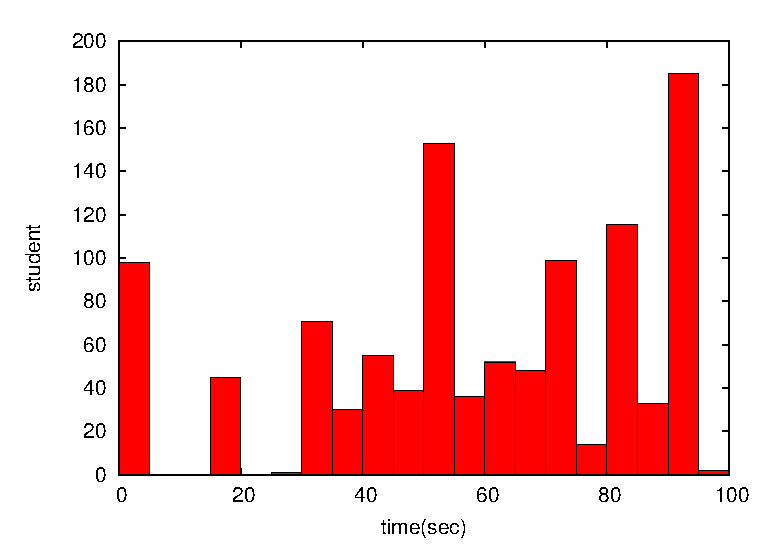
\includegraphics[bb=0 0 390 248,clip,scale=1.0]{oMo12_hist.eps}
 \hspace{-10mm} 
\vspace{-5mm}
  \caption{移動時間ごとの学生数(春学期月曜午前)}
  \label{omo12}
 \end{center}
\end{figure}

表\ref{j:normal_information}は,本実験1での実験結果である.
表\ref{j:normal_information}より,本実験1では,全ての曜限において,比較的短い計算時間で最大の移動時間の最小値を求めることができた.
また,先行研究の結果(表\ref{senkou_kekka})と比べて,制約数は遥かに小さくなっていることがわかる.
さらに,変数についても,全ての曜限において,最低でも半分以下になっている.
これらの要因によって,本実験1では,短い計算時間で解を得ることができたと考えられる.

図\ref{omo12}は,春学期月曜午前における,移動時間(5秒ごと)制の学生数を表している.
これより,学生の一部は移動時間が大きいが,全体的にはある程度移動時間が短くなるような教室割当が求められていることがわかる.
これらのことより,本実験1では,期待した実験結果を得ることができたといえる.

\subsection{本実験2:移動時間の最小値が大きい授業を取り除いた実験}
表\ref{j:normal_information}より,春学期月曜午後,及び春学期木曜午後の最大移動時間の最小値が,他よりもかなり大きいことがわかる.
この原因を調べたところ,ある特定の授業の移動時間が大きい,ということがわかった.
そこで,本実験2として,その授業を除外し,結果がどのように変わるかを調べる実験を行った.

\begin{table}[H]
\caption{本実験2の結果}
\label{jikken2_kekka}
\vspace{-5.0mm}
\begin{center}
\begin{tabular}{|r|cccccc|}
\hline
\multicolumn{1}{|c|}{曜限} & 最大(秒) & 平均(秒) & 制約数 & 変数の数 & nonzeros & 計算時間(秒)\\
\hline
春学期月曜午後  & 68 & 37.9 & 2530 & 2290 & 30761 &  13.54\\
      木曜午後  & 51 & 15.4 & 792  & 910  & 10088 &   1.84\\
\hline
\end{tabular}
\end{center}
\end{table}

\if0
\begin{figure}[htpb]                        
\begin{minipage} {0.5\hsize}                             
\begin{center}                              
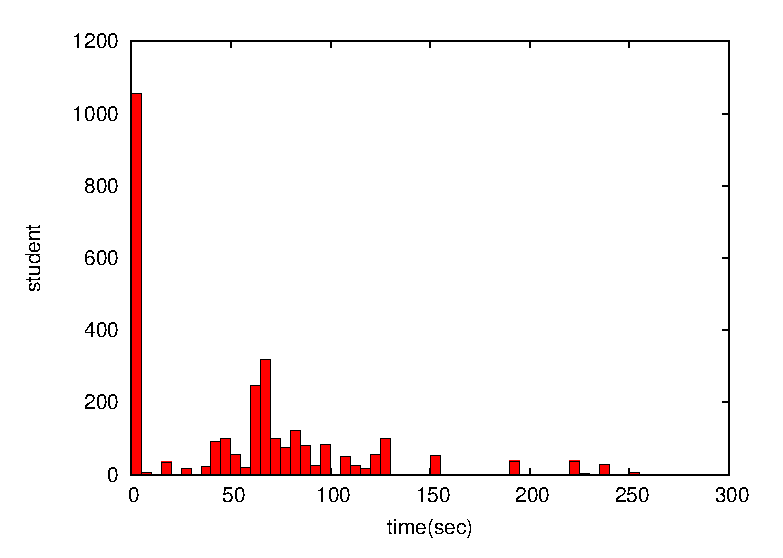
\includegraphics[bb=0 0 390 248,clip,width=\hsize]{oMo345_hist.eps}   
本実験1:春学期月曜午後
\end{center}                                    
\end{minipage}                                 
\begin{minipage}{0.5\hsize}                                            
\begin{center}                              
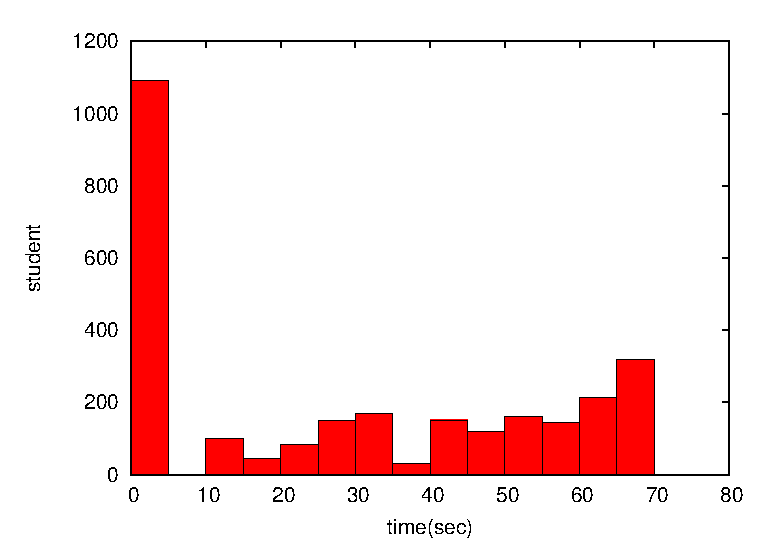
\includegraphics[bb=0 0 390 248,clip,width=\hsize]{oMo345_2_hist.eps}   
本実験2:春学期月曜午後
\end{center}                                    
\end{minipage}                                 
\caption{春学期月曜午後における本実験1と本実験2の移動時間ごとの学生数の比較}                              
\label{hikaku1-2}                                
\end{figure}                                 
\fi

\begin{figure}[thpb]
 \begin{center}
 \hspace{5mm} 
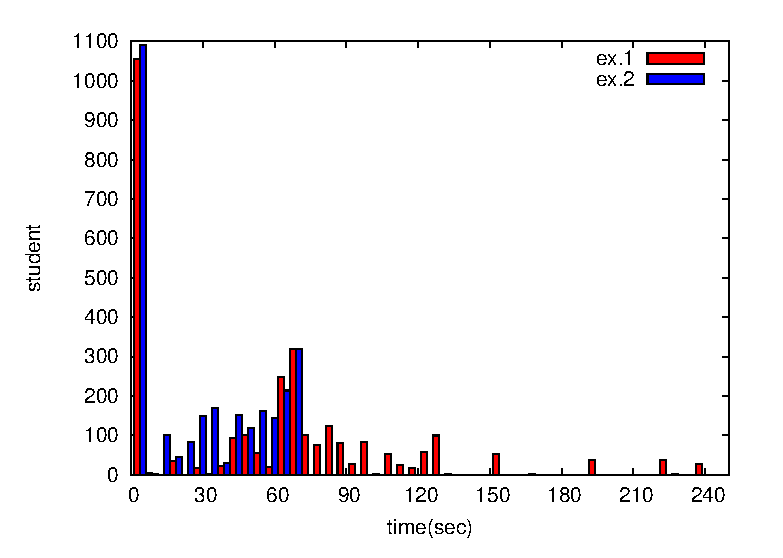
\includegraphics[bb=0 0 390 248,clip,scale=1.0]{omonagahist.eps}
 \hspace{-10mm} 
\vspace{-5mm}
\caption{春学期月曜午後における本実験1と本実験2の移動時間ごとの学生数の比較}                              
  \label{hikaku1-2}
 \end{center}
\end{figure}

表\ref{jikken2_kekka}は,本実験2の実験結果である.
表\ref{jikken2_kekka}より,いずれの曜限における移動時間の最大値とも,本実験1におけるその他の曜限の結果に近い値になっており,特定の授業だけが移動に時間を要していたということが確認できた.
また,図\ref{hikaku1-2}は,春学期月曜午後における本実験1と本実験2の,移動時間(5秒ごと)制の学生数のを比較した図である.
図\ref{hikaku1-2}より,特定の授業を除外することで,その他の授業間の移動時間を大幅に短くできていることがわかる.
この結果より,移動時間が大きくなりそうな授業の教室割当をあらかじめ決めておき,その後に提案手法により残りの授業の教室割当を決めれば,よい割当が求められることがわかる.

\subsection{本実験3:希望教室を設定した実験}
本実験3は,春学期火曜午前のデータに考慮制約2の希望教室を設定して行った実験である.
3つの授業 60190\_oTu1\_1, 60272\_oTu1\_1, 60273\_oTu1\_1にそれぞれ2つの教室4-101,4-102を希望教室として設定している.
すなわち,3つ全ての授業の希望が叶うことはない状況を設定している.

\begin{table}[H]
\caption{春学期火曜午前における本実験1と本実験3の結果の比較}
\label{l:normal_information}
\begin{center}
\begin{tabular}{|r|cccccc|}
\hline
\multicolumn{1}{|c|}{実験} & 最大(秒) & 平均(秒) & 制約数 & 変数の数 & nonzeros & 計算時間(秒)\\
\hline
本実験1       & 76  & 39.4 & 1753 & 2150 & 28679 &  1.04\\
本実験3       & 76  & 47.9 & 1753 & 2150 & 28679 &  1.73\\
\hline
\end{tabular}
\end{center}
\end{table}

\if0
\begin{figure}[htpb]                        
\begin{minipage} {0.5\hsize}                             
\begin{center}                              
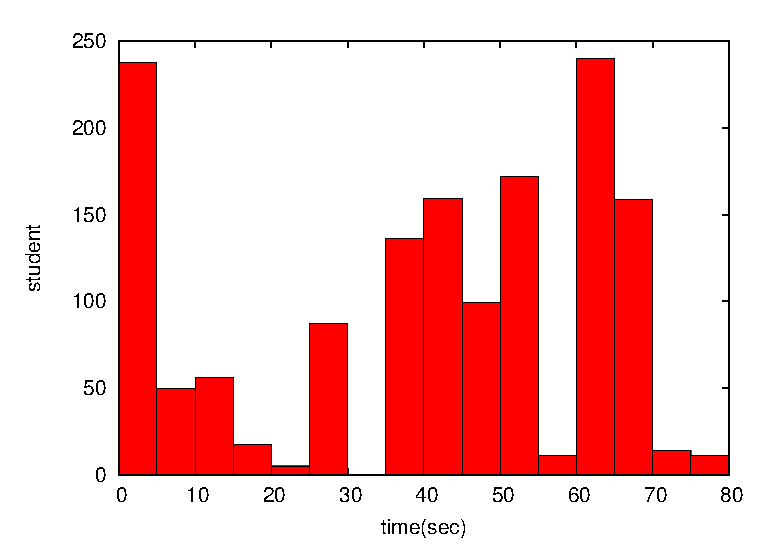
\includegraphics[bb=0 0 390 248,clip,width=\hsize]{oTu12_hist.eps}   
本実験1:春学期火曜午前
\end{center}                                    
\end{minipage}                                 
\begin{minipage}{0.5\hsize}                                            
\begin{center}                              
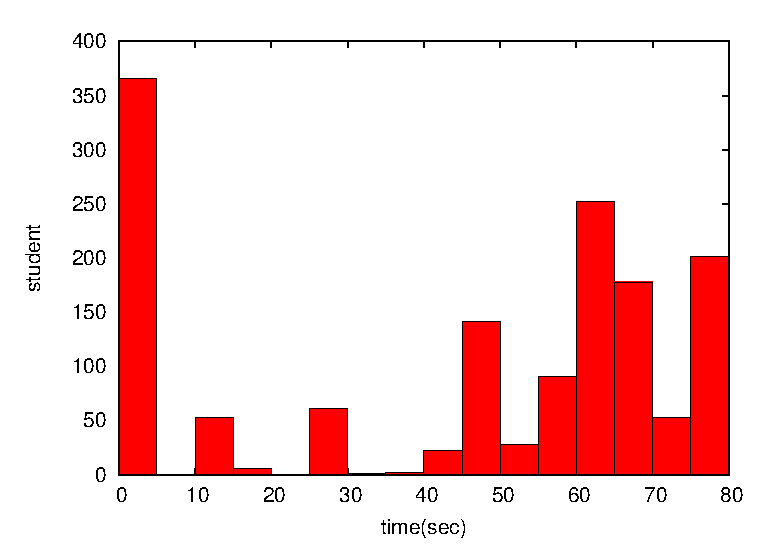
\includegraphics[bb=0 0 390 248,clip,width=\hsize]{oTu12_2_hist.eps}   
本実験3:春学期火曜午前
\end{center}                                    
\end{minipage}                                 
\caption{春学期火曜午前における本実験1と本実験3の移動時間ごとの学生数の比較}                              
\label{hikaku1-3}                                
\end{figure}                                 
\fi

\begin{figure}[thpb]
 \begin{center}
 \hspace{5mm} 
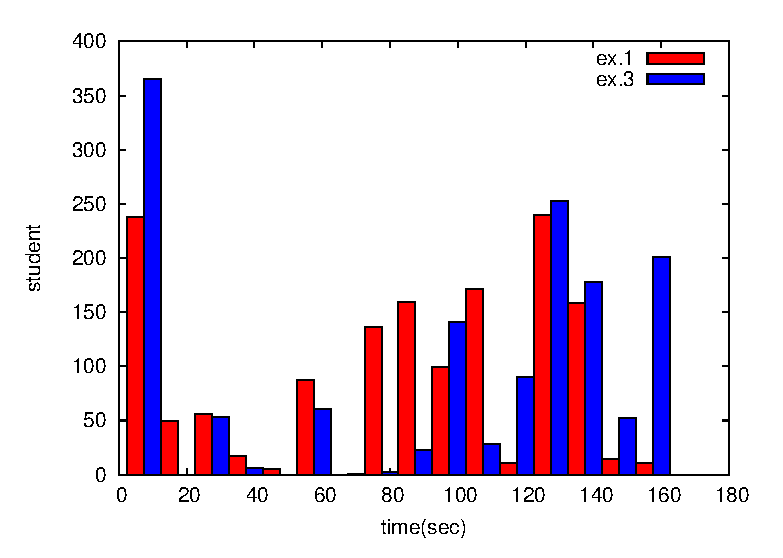
\includegraphics[bb=0 0 390 248,clip,scale=1.0]{otukarehist.eps}
 \hspace{-10mm} 
\vspace{-5mm}
\caption{春学期火曜午前における本実験1と本実験3の移動時間ごとの学生数の比較}                              
  \label{hikaku1-3}
 \end{center}
\end{figure}

表\ref{l:normal_information}は,本実験3の実験結果である.
表\ref{l:normal_information}より,最大の移動時間の最小値は本実験1と同じ値であるが,平均移動時間については本実験1の結果より8.5秒大きくなっていることがわかる.
これは,希望教室を叶えることで,最大の移動時間の最小値には影響しないが,移動が発生してしまったと考えられる.
図\ref{hikaku1-3}は,春学期火曜午前における本実験1と本実験3の,移動時間(5秒ごと)制の学生数のを比較した図である.
図\ref{hikaku1-3}より,移動時間が0秒の学生数も増加しているが,同時に移動時間が大きくなってしまう学生数も増加していることがわかる.
また,目的関数の値を確認すると,希望教室を最大限叶えることができていることがわかった.
この結果より,事前に希望を調べておき,それをできるだけ叶えるような教室割当が求められることがわかった.



\if0
\section{考察}
最大の移動時間を最小化するという方法によって,最大の移動時間を小さくすることができた.
これは,移動時間の最小化をすることができたといえるだろう.
3つの実験によって,本研究のモデルを用いることにより,様々な状況に対応することができるだろう,ということがわかる.
\fi
%\end{document}
